\chapter{Systemmodell}
Die Rechteverwaltung basiert auf \glspl{Gruppe}. Jede Gruppe hat verschiedene Berechtigungen. Im Folgenden wird zwischen Reviewern, Nutzern und Administratoren unterschieden. 
Es wird bei der Ansicht der Workflows nicht zwischen Nutzern, Reviewern und Admins unterschieden. 

Reviewer können sich anmelden, abgeschlossene Workflows einsehen und aktuell laufende Workflows einsehen.

Nutzer können /M10/, /M20/, /M30/ und alle Funktionalitäten, die Reviewer nutzen können, nutzen.

Admin Nutzer kann die Funktionen /FA260/, /FA270/, /FA280/, /FA290/ und alle Funktionen, die Nutzer und Reviewer ausführen können, ausführen.

%Nochmal am Ende anschauen und links fixen

\begin{figure}[ht]
    \centering
    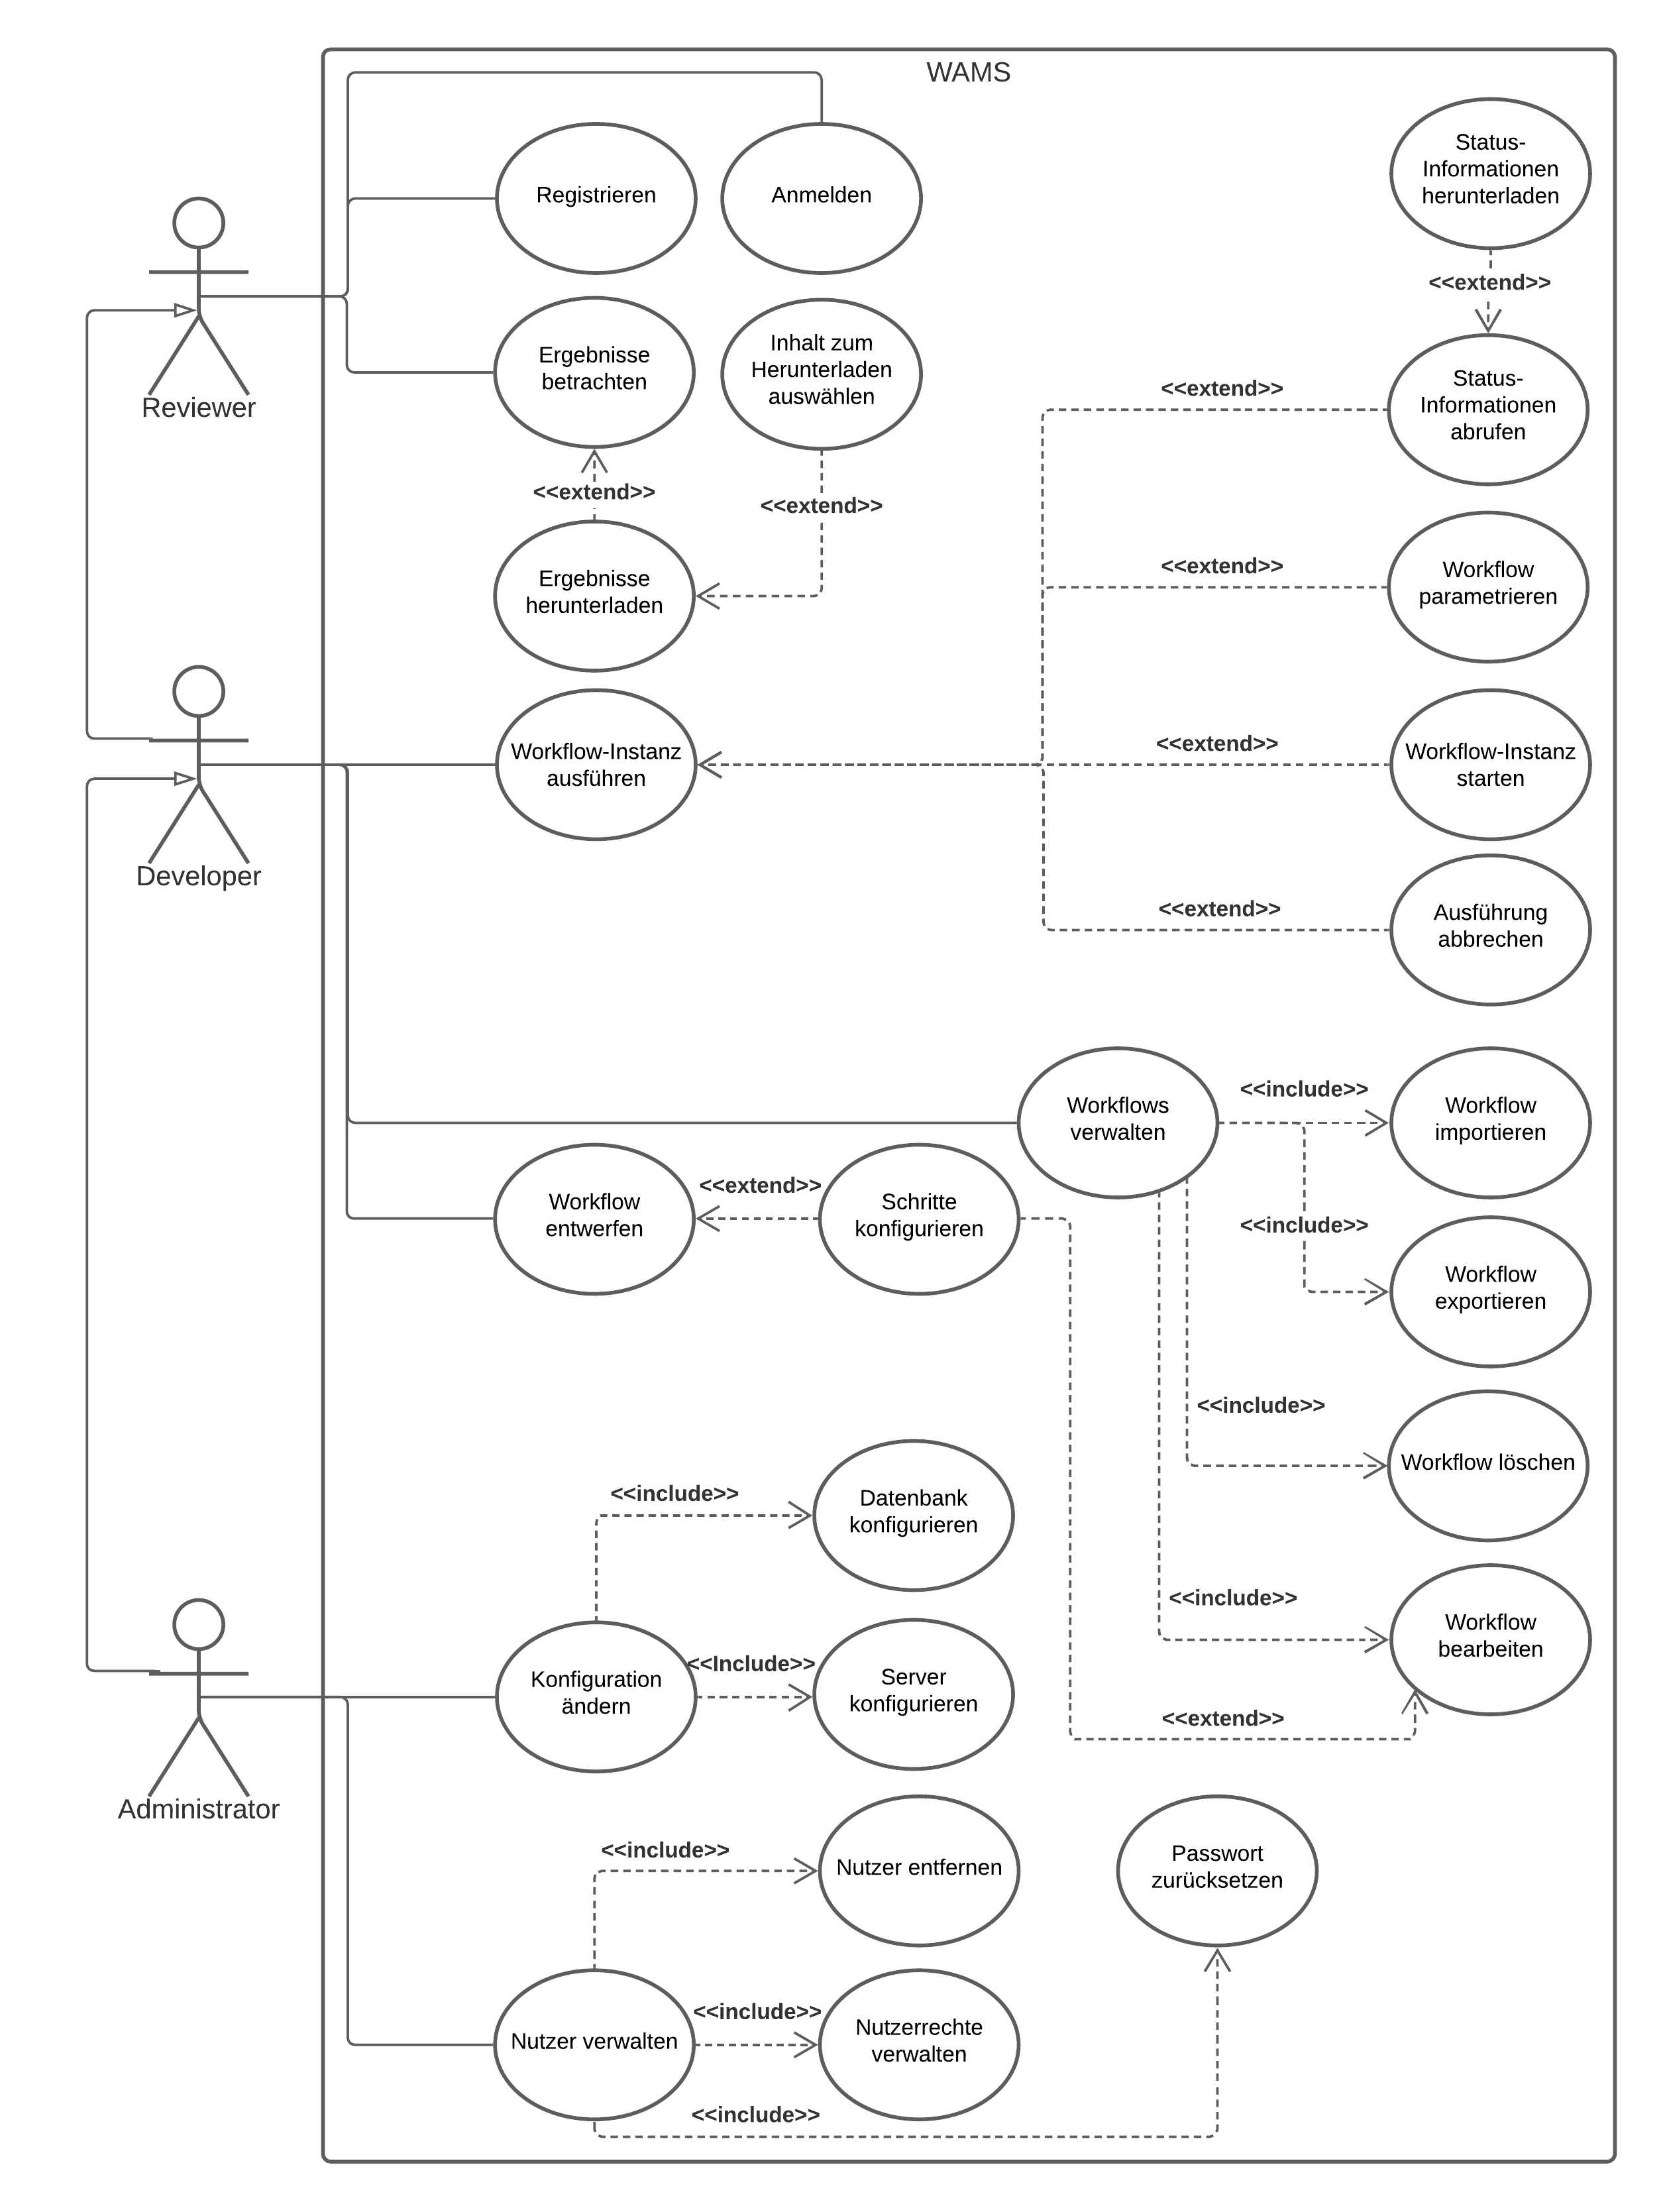
\includegraphics[width = \textwidth]{Grafiken/Diagramme/Anwendungsfalldiagramm.png}
    \caption{Anwendungsfälle und Verteilung der Rechte und nutzbarer Funktionen}
    \label{fig:Abb 1}
\end{figure}